%% ------------------------------------------------------------
%% TITLE:       Probability and Statistics For Bioengineers - Formula Summary 
%% AUTHORS:     BINGHUAN W LI (Dept. Chemical Eng/Bio Eng, Imperial)
%%              PETER Y XIE (Dept. Mechanical Eng, Stanford)
%  GRAPHS:      By courtesy of Dr Joseph van Batenburg-Sherwood 
%% COMPILED:    XeLaTeX with TeX Live version 2023
%% LICENSE:     This work is licensed under a Creative Commons Attribution-NonCommercial 4.0 International License.
%% ------------------------------------------------------------

% Version History:
% v1.0  - 2022-01-03 - Initial draft
% v1.1  - 2022-06-28 - Fixed typos
% v1.1  - 2024-11-09 - Fixed typos


\documentclass{article}
\usepackage[sfdefault]{arimo} 
\usepackage[top=2cm, bottom=1cm, left=2cm, right=2cm]{geometry}

% set math env
\usepackage{amsmath, amsfonts, mathrsfs, mathtools, amssymb}
\usepackage{changepage}

\usepackage{graphics, float}

% table scaling
\usepackage{adjustbox}

% write pdf metadata
\usepackage{hyperref}
\usepackage[usenames,dvipsnames]{xcolor}
\definecolor{linkcolour}{RGB}{0,62,116}
\hypersetup{pdfauthor={Li, Binghuan},
            pdftitle={Probs-and-Stats, Formula Sheet},
            pdfsubject={last update date: \today},
            colorlinks,breaklinks,
            urlcolor=linkcolour, 
            linkcolor=linkcolour}
            
% env to insert external pdf 
\usepackage{pdfpages}

\usepackage{booktabs}

\usepackage{framed}

% set section title size
\usepackage{titlesec}
\titleformat*{\section}{\large\bfseries}
\titleformat*{\subsection}{\normalsize\bfseries}
\titleformat*{\subsubsection}{\small\bfseries}

% caption setting env
\usepackage{caption}
\captionsetup[table]{labelformat=empty}

% set header/footer
\usepackage{fancyhdr}
\pagestyle{fancy}
\fancyhf{}
\lhead{\textit{Probability and Statistics for Bioengineering - Formula Sheet}}
\rhead{\thepage}


%%%%%%%%%%%%%%%%%%%%%%%%%%%%%%%%%%%%%%%%%%%%%%%
\begin{document}

\section{Mean, Median and Standard Deviation}

\begin{table}[H]
    \centering
    \begin{adjustbox}{width=\columnwidth,center}
    \begin{tabular}{c| c| c | c}
        Mean & Median & Standard Deviation & MAD\\ [0.7ex] \hline 
        $\displaystyle \bar{x}=\frac{1}{n}\sum_{i=1}^{n}x_{i} = \frac{x_{1}+x_{2}+...+x_{n}}{n}$ & 
        $\Tilde{x} = \begin{cases} 
        x(\frac{n+1}{2}), & n \ \text{is odd} \\
        0.5(x(\frac{n}{2})+x(\frac{n}{2}+1)), & n \ \text{is even}
        \end{cases}$ &
        $\displaystyle s = \sqrt{\frac{1}{n-1}\sum_{i=1}^{n} (x_{i}-\bar{x})^{2}}$
        & $\displaystyle MAD = k|\widetilde{x_{i} - \hat{x}}|$ \\
          &  &  &  $k = 1.4826$ \footnotesize{(normal)}\\
    \end{tabular}
    \end{adjustbox}
\end{table}

\begin{itemize}
    \item[-] $s$, $s^{2}$ and $\bar{x}$ denote \underline{sample} S.D., variance and mean.
    \item[-] $\sigma$, $\sigma^{2}$ and $\mu$ denote \underline{population} S.D., variance and mean \footnote{Mean is simply the average value of a \textit{given sample}. Expect value is used when we want to calculate the mean of a \textit{probability distribution}.}.\\
    
    \item[-] \textbf{Trimmed Mean at $p\%$} - Remove $p/2$ percentile from both ends of the data and calculate the mean
    \item[-] \textbf{Standard Error on the mean} - 
    $\displaystyle S_{\bar{X}} = \frac{S_{X}}{\sqrt{n}}$, where $n$ is the sample size, $S_{X}$ is the standard deviation
\end{itemize}

%%%%%%%%%%%%%%%%%%%%%%%%%%%%%%%%%%%%%%%%
\section{Probability Theory}
\subsection*{Set Theory}
\begin{table}[H]
    \centering
    \begin{adjustbox}{width=\columnwidth,center}
    \begin{tabular}{c| c| c |c}  
        Union & Intersection & Complement & Relative Complement\\ [0.7ex] \hline \vspace{1ex}
       A \underline{OR} B & A \underline{AND} B & \underline{NOT} A & A \underline{AND} \underline{NOT} B \\
       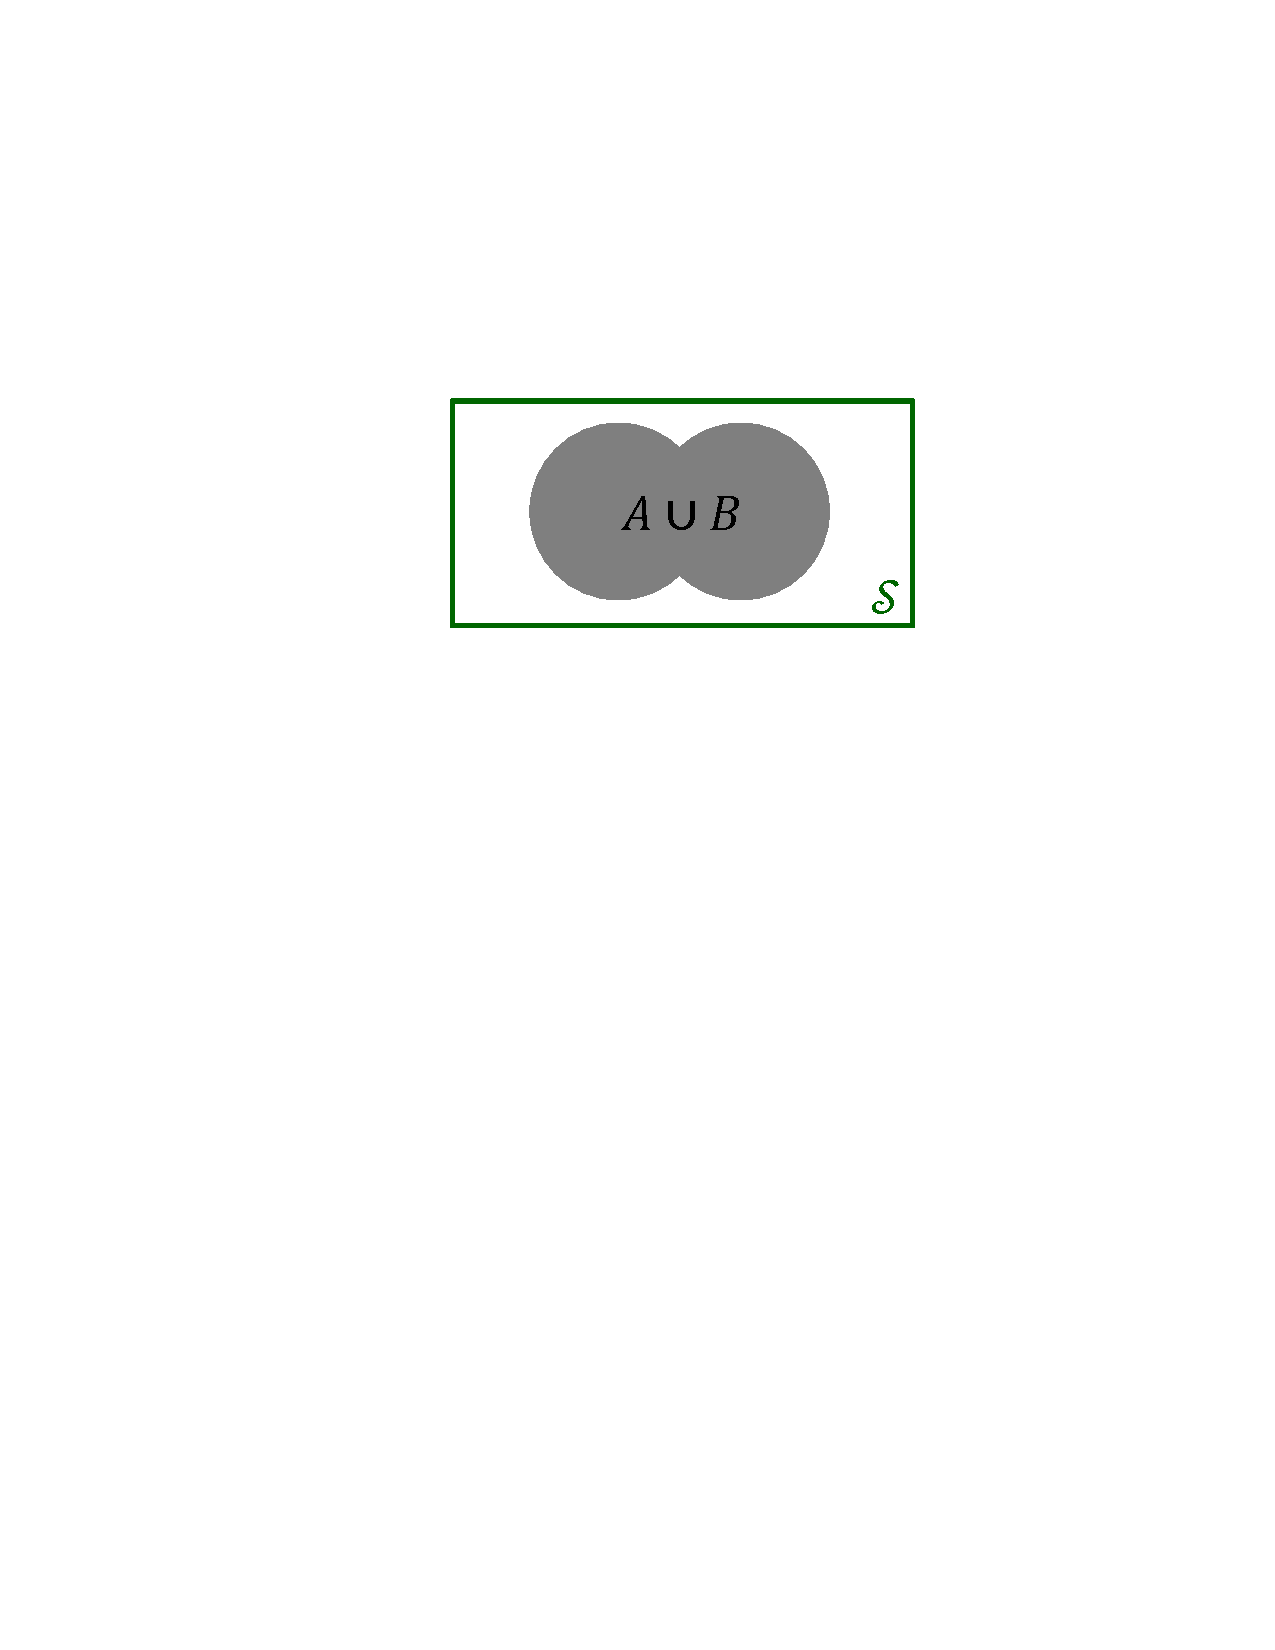
\includegraphics[width=0.2\textwidth]{./images/AorB.pdf}&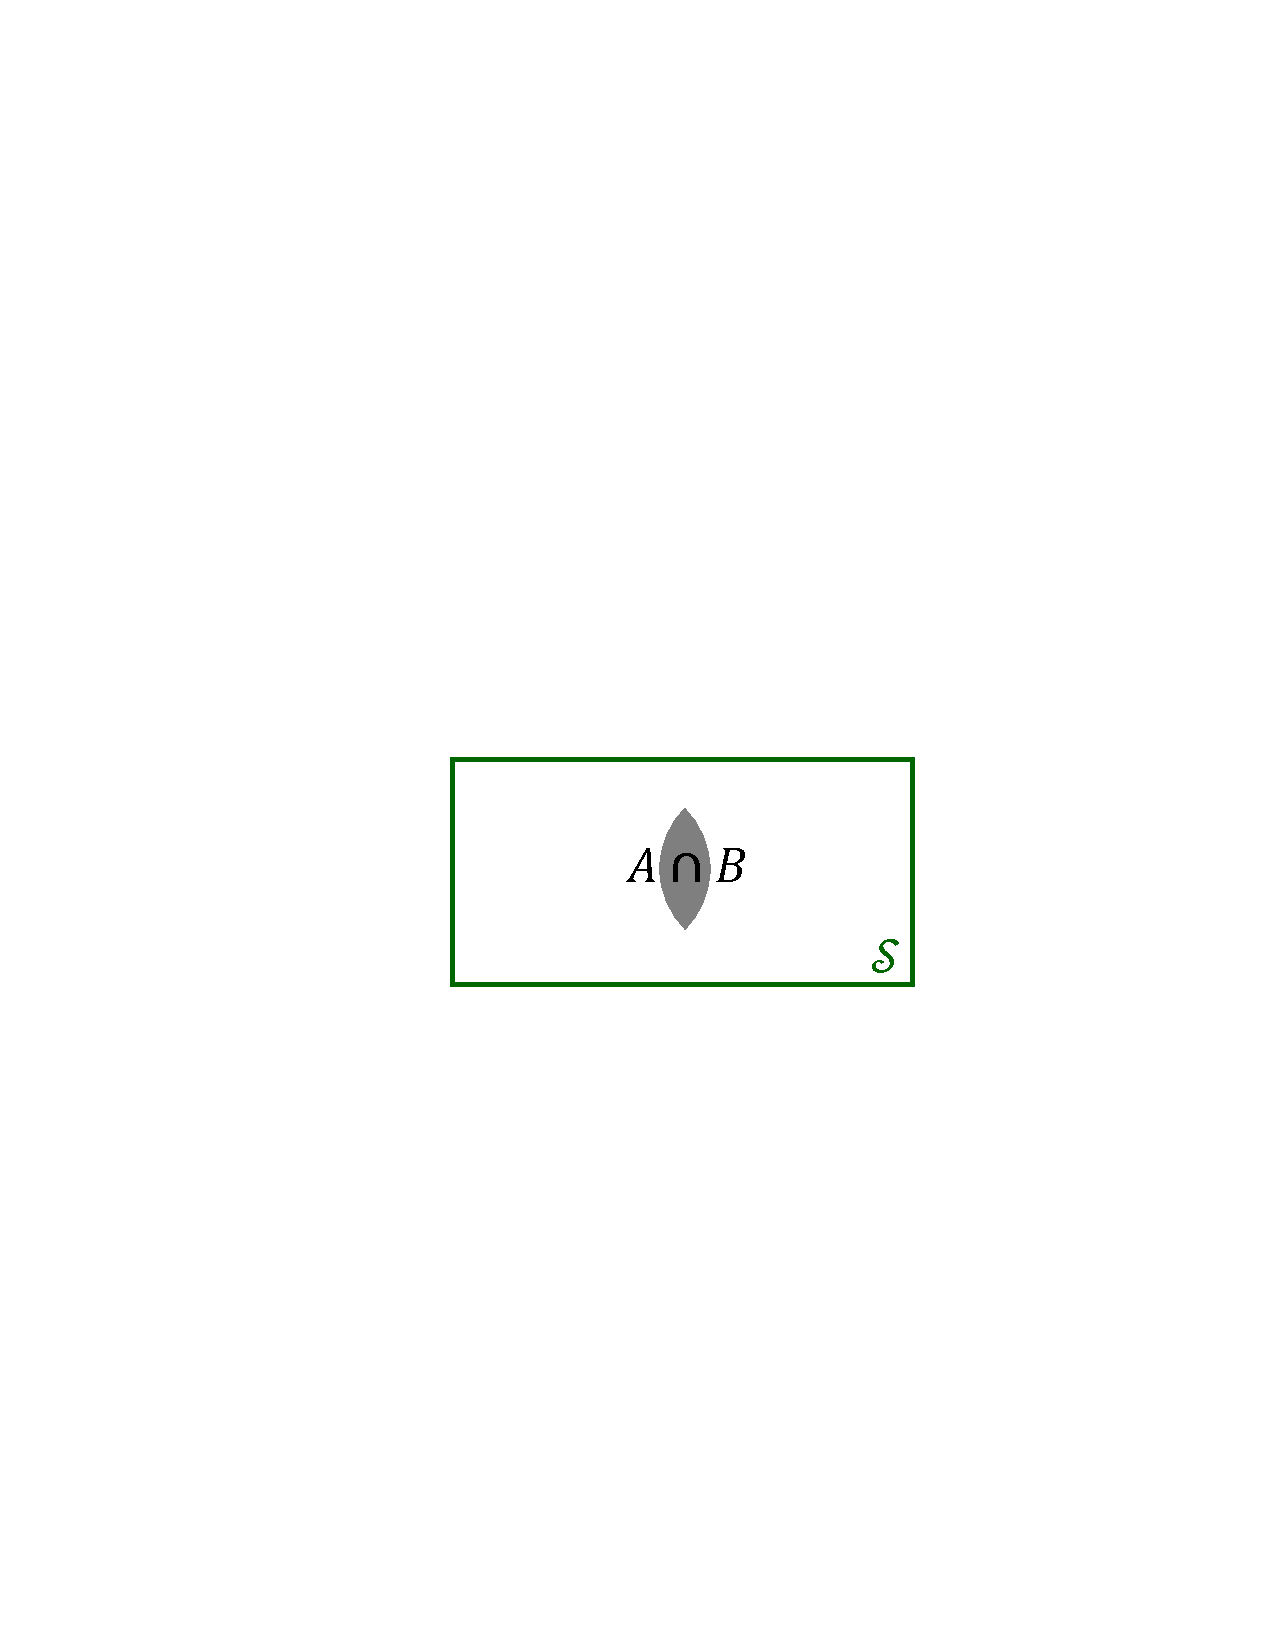
\includegraphics[width=0.2\textwidth]{./images/AandB.pdf}&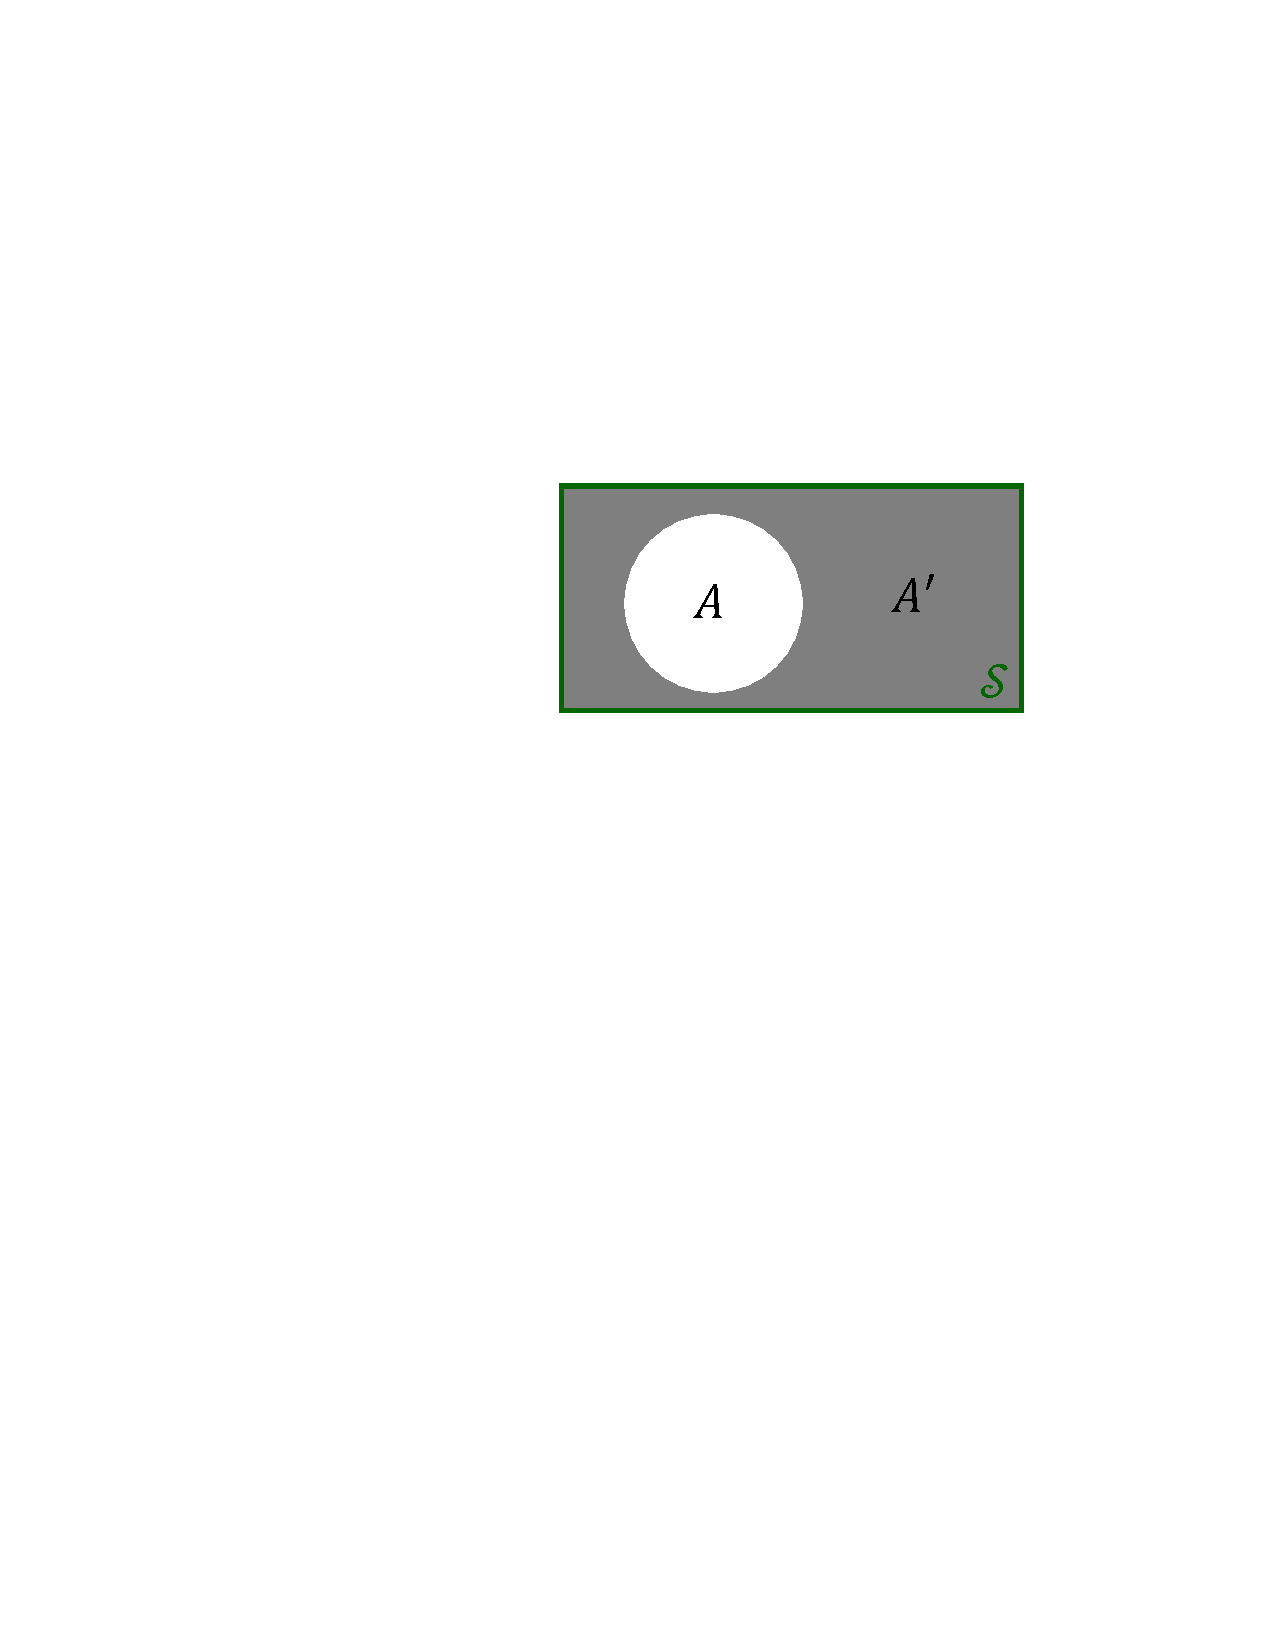
\includegraphics[width=0.2\textwidth]{./images/notA.pdf}&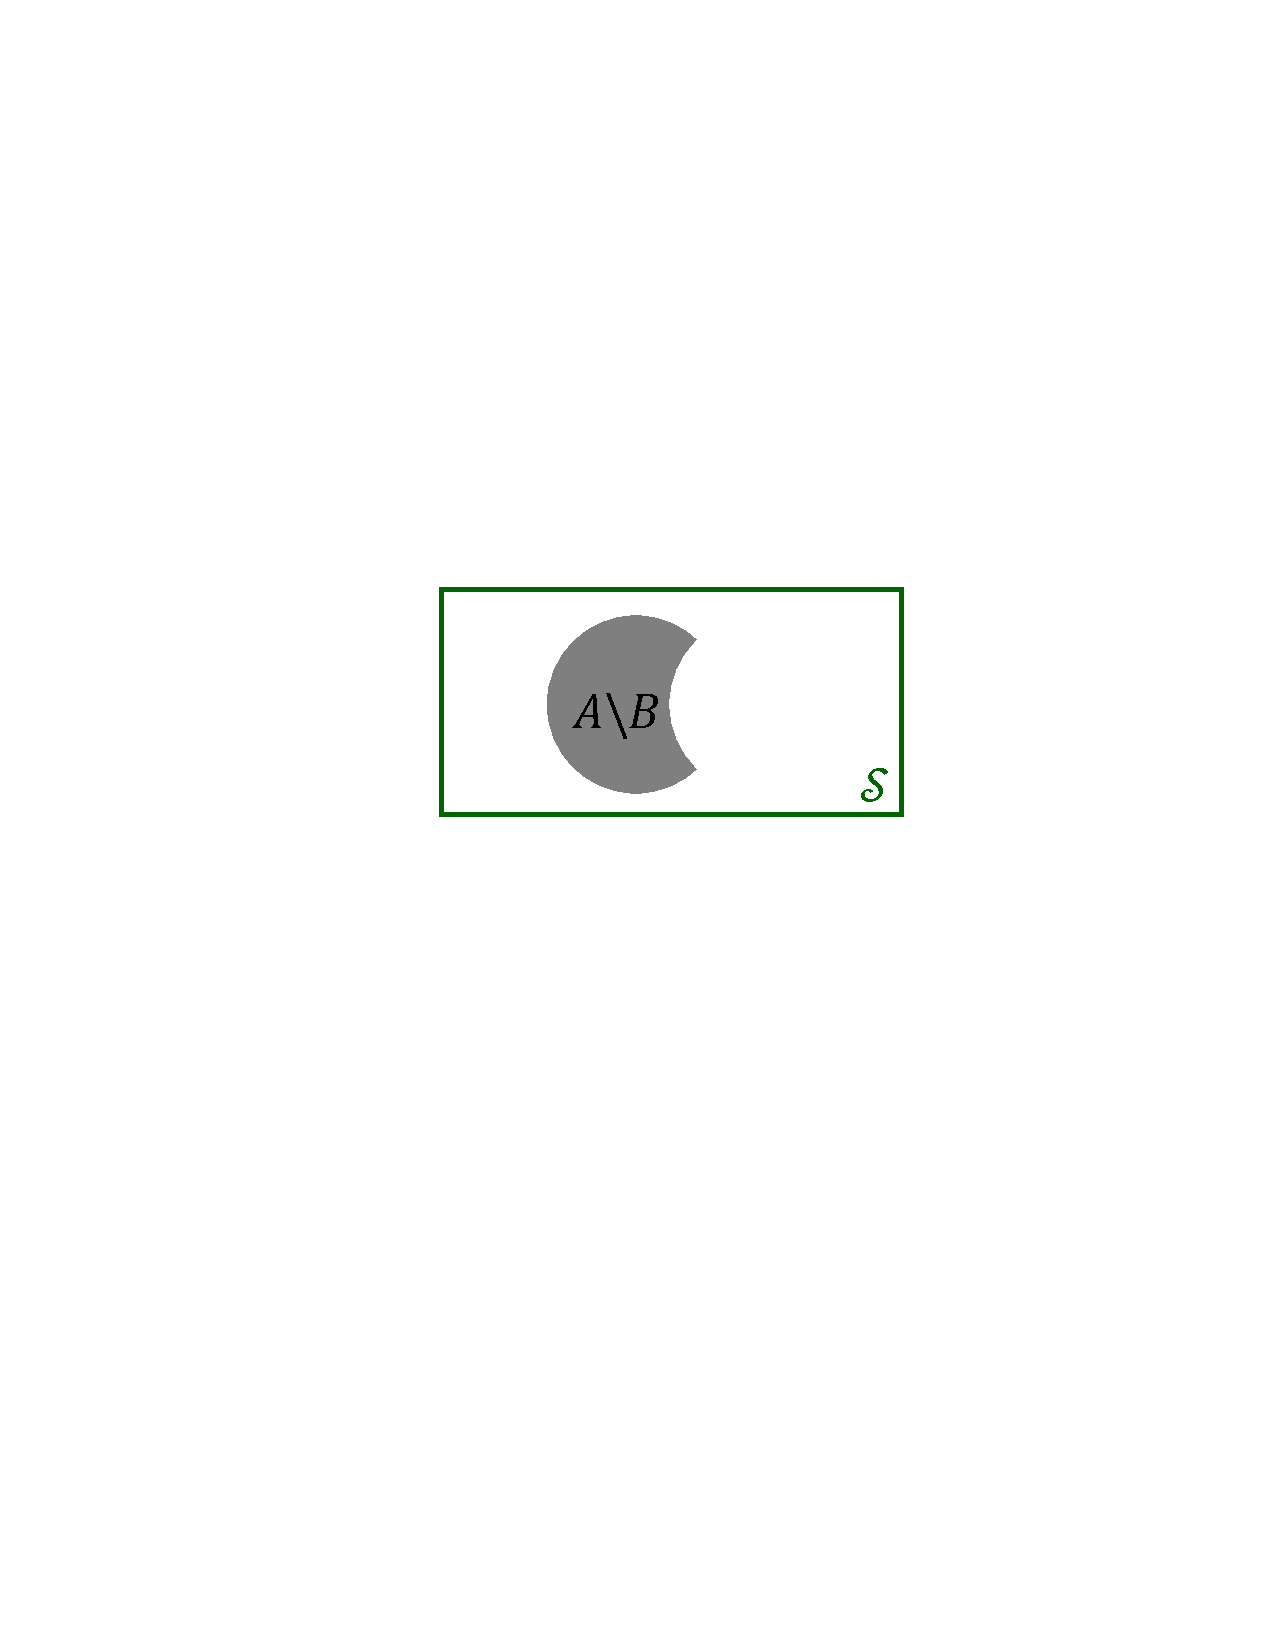
\includegraphics[width=0.2\textwidth]{./images/Aand_notB.pdf}\\
       $P(A\cup B) = P(A)+P(B)-P(A\cap B)$ &&$P(A') = 1 - P(A)$ &
    \end{tabular}
    \end{adjustbox}
\end{table}

%%
\subsection*{Counting}
\begin{itemize}
\item Product Rule - $\displaystyle n = n_{1}\times n_{2}\times n_{3}\times...\times n_{k}$
    \item Permutations: Ordered, dependent selections (without replacement) -
    $\displaystyle P_{k,n} = \frac{n!}{(n-k)!}$
    \item Combinations: Unordered selections (without replacement) - 
    $\displaystyle C_{k,n} = \frac{P_{k,n}}{k!} = {n \choose k} = \frac{n!}{k!(n-k)!}$
\end{itemize}

%%
\subsection*{Conditional Probability}
\begin{itemize}
    \item Conditional probability: knowing that A has happened, the probability of B given A - $\displaystyle P(B|A) = \frac{P(B \cap A)}{P(A)}$
    \item Bayes Theorem - $\displaystyle P(A_{j}|B) = \frac{P(B|A_{j})P(A_{j})}{\sum_{i=1}^{k}P(B|A_{i})P(A_{i})} $\\\\
    (Applies if events A are mutually exclusive and exhaustive (defines the whole set)).
\end{itemize}

%%
\subsection*{Independence}
\begin{itemize}
    \item Independent: event A is unaffected by event B
    \[P(A\cap B)=P(A)P(B) \quad \Rightarrow \quad P(A|B) = P(A), \quad\quad P(B|A) = P(B)\]
\end{itemize}


%%%%%%%%%%%%%%%%%%%%%%%%%%%%%%%%%%%%%%%%%%%%%%%%

\section{Probability Distributions and Discrete Random Variables}
\subsection*{Binomial and Poisson Distribution}
\begin{minipage}{.8\textwidth}
\begin{table}[H]
    \centering
    \begin{tabular}{l c c}  
        & Binomial Distribution & Poisson Distribution\\ [0.7ex] \hline \vspace{1ex}
        Probability Density Function & $ \displaystyle b(x;n,p) ={ n \choose x} p^{x}(1-p)^{n-x}$  & $\displaystyle po(x,\lambda) = \frac{e^{-\lambda}\lambda^{x}}{x!}$  \\ [0.5ex]
        Expected Value, $E(x)$ & $E(x) = np$ & $E(x) = \lambda$\\ [0.5ex] 
        Variance, $V(x)$ & $\displaystyle V(x) = np(1-p) = npq$ & $\displaystyle V(x) = \lambda(1-\frac{\lambda}{n})\approx \lambda$  \\ [0.5ex] 
    \end{tabular}
\end{table}
\end{minipage}
\begin{minipage}{.2\textwidth}
\begin{framed}
Note: \\\\
$V(x)$ can also be expressed as $V(x)=E(x^{2})-(E(x))^{2}$.    
\end{framed}

\end{minipage}

%%
\subsection*{Discrete Random Variables}
% \begin{adjustwidth}{-100pt}{-100pt}
\begin{table}[H]
    \centering
    \begin{adjustbox}{width=\columnwidth,center}
    \begin{tabular}{c| c| c}  
        Bernoulli RV & Expected Value & Variance\\ [1.0ex] \hline 
        $p(x;\alpha) = \begin{cases}
        1-\alpha, & if \ x=0 \\
        \alpha, & if \ x=1\\
        0, & otherwise
        \end{cases}$
        &
        $\displaystyle E(x)=\mu_{X}=\sum_{x\in D}xp(x)$
        &
        $\displaystyle V(X) = \sigma_{X}^{2}=\sum_{x\in D}(x-\mu_{X})^{2}p(x)=E[(X-\mu_{X})^{2}]$
    \end{tabular}
    \end{adjustbox}
\end{table}

%%%%%%%%%%%%%%%%%%%%%%%%%%%%%%%%%%%%%%%%%%%%%%%%
\section{Continuous Random Variables and Joint Probability}
\subsection*{Random Variables}
\begin{table}[H]
    \centering
    \begin{tabular}{|l|c|}
    \hline
     \addlinespace[.3ex] Probability density function & $\displaystyle P(a \leq X \leq b) = \int_{a}^{b}f(x)dx$ \\ [.5ex] \hline
    \addlinespace[.3ex] Cumulative distribution function & $\displaystyle F(x) = P(X\leq x) = \int_{-\infty}^{x} f(y)dy \  \text{and} \ \int_{-\infty}^{+\infty} f(x)dx = 1$ \\ [.5ex] \hline
    \addlinespace[.3ex] Expected value & $\displaystyle \mu_{X} = E(X) = \int_{-\infty}^{+\infty} xf(x) dx$ \\ [.5ex] \hline 
    \addlinespace[.3ex] Variance & $\displaystyle \sigma_{X}^{2} = V(X) = \int_{-\infty}^{+\infty} (x-\mu)^{2}f(x) dx$ \\ [.3ex] \hline
    \end{tabular}
\end{table}

\subsection*{Joint Probability Distributions}
\begin{itemize}
    \item Discrete Joint random variables
    \begin{table}[H]
    \centering
    % \begin{adjustbox}{width=\columnwidth,center}
    \begin{tabular}{c| c| c}  
        Joint probability mass function (PMF) & Expected Value & Marginal PMFs\\ [0.7ex] \hline 
        \addlinespace[.4ex] $p(x,y)=P(X=x$ and $Y=y)$ 
        & 
        $\displaystyle E[h(X,Y)]=\sum_{X}\sum_{Y}h(x,y)p(x,y)$
        &
        $P_{X}(x)=\sum_{y}p(x,y)$\\ 
        
        $\sum_{x}\sum_{y}p(x,y)=1$
        &
        &
        $P_{Y}(y)=\sum_{x}p(x,y)$\\ 
    \end{tabular}
\end{table}

    \item Continuous Joint random variables
    \begin{table}[H]
    \centering
   \begin{adjustbox}{width=\columnwidth,center}
    \begin{tabular}{c| c| c}  
        Joint probability mass function (PDF) & Expected Value & Marginal PDFs\\ [0.7ex] \hline 
        \addlinespace[.4ex] $\displaystyle P[(X,Y)\in A]=\int\int_{A} f(x,y) dx dy$
        &
        $\displaystyle E[h(X,Y)]=\int_{-\infty}^{+\infty}\int_{-\infty}^{+\infty}h(x,y)f(x,y)dx dy$
        & 
        $\displaystyle f_{X}(x)=\int_{-\infty}^{+\infty} f(x,y)dy$ \\ [2ex]
        
        &
        $\displaystyle P[a\leq X\leq b, c \leq Y \leq d]=\int_{c}^{d}\int_{a}^{b}f(x,y)dx dy$
        & 
        $\displaystyle f_{Y}(y)=\int_{-\infty}^{+\infty} f(x,y)dx$
    \end{tabular}
    \end{adjustbox}
\end{table}
\end{itemize}

\vspace{-1cm}
\subsection*{Independence}
$X$ and $Y$ are independent if for every pair $x, y$:
\begin{itemize}
    \item Discrete: \quad $p(x,y) = p_{x}(x)p_{y}(y)$
    \item Continuous: \quad $f(x,y) = f_{x}(x)f_{y}(y)$
\end{itemize}

%%%%%%%%%%%%%%%%%%%%%%%%%%%%%%%%%%%%%%%%%%%%%%%%

\section{Normal Distribution}

\begin{minipage}{0.7\textwidth}
\begin{itemize}
    \item Probability Density Function (pdf):\[f(x) = \frac{1}{\sqrt{2\pi \sigma^{2}}}e^{-\frac{(x-\mu)^{2}}{2\sigma^{2}}}\]
    \item Cumulative Distribution Function (cdf): \[F(X) = \frac{1}{2}\bigg[ 1+ \text{erf}\bigg( \frac{x-\mu}{\sqrt{2\sigma^{2}}} \bigg) \bigg]\]
    where \[\text{erf}(x) = \frac{2}{\sqrt{\pi}} \int_{0}^{x} e^{-t^{2}}dt\]
\end{itemize}
\end{minipage}\hfill
\begin{minipage}{0.3\textwidth}
\begin{table}[H]
    \centering
    \begin{tabular}{l c}\hline
        Discrete & Continuous \\ \hline
        $X=A$ & $A-0.5 < Y < A+0.5$\\ 
        $X\leq A$ & $Y<A+0.5$\\ 
        $X<A$ & $Y<A-0.5$ \\
        $X\geq A$ & $Y>A-0.5$ \\
        $X>A$ & $Y>A+0.5$ \\
    \end{tabular}\caption{Continuity Correction - Normal approximation of discrete distributions (e.g. Binomial)}
\end{table}
\end{minipage}

%%
\subsection*{Standard Normal Distribution}
Standard normal distribution is a special case of normal distribution with $\mu = 0$ and $\sigma =1$.
\begin{table}[H]
    \centering
    \begin{tabular}{c|c}
        Probability Density Function (PDF) &  
        Cumulative Distribution Function (CDF)\\ \hline
        $\displaystyle f(Z) = \frac{1}{\sqrt{2\pi }}e^{-\frac{z^{2}}{2}}$ & 
        $\displaystyle \Phi(z) = F(Z) = \frac{1}{2}\bigg[ 1+ \text{erf}\bigg( \frac{z}{\sqrt{2}} \bigg) \bigg]$ and \ $\displaystyle Z = \frac{X-\mu}{\sigma}$
    \end{tabular}
\end{table}


%%
\subsection*{Central Limit Theorem}
For sufficiently large n:
\begin{itemize}
    \item Mean sample mean is the population mean - $\displaystyle E[\bar{X}] = \mu_{\bar{X}} = \mu$
    \item Sample mean variance decreases as sample size increase - $\displaystyle  V[\bar{X}] = \sigma_{\bar{X}}^{2} = \frac{\sigma^{2}}{n}$
    \item Standard error on the mean (SEM) is the SD of sample means - $\displaystyle \sigma_{\bar{X}} = \frac{\sigma}{\sqrt{n}}$
\end{itemize}

%%
\subsection*{Margin of Error, Confidence Intervals}
Unknown $\sigma$, large $n$.
\begin{table}[H]
    \centering
    \begin{tabular}{c|c}
        Confidence interval (CI) &  
        Margin of Error (ME)\\ \hline
        $\displaystyle CI = \bar{X} [\bar{X_{l}}, \bar{X_{u}}] \ =\  \bigg[\bar{X}-Z_{\frac{\alpha}{2}}\frac{\sigma}{\sqrt{n}},\ \bar{X}+Z_{\frac{\alpha}{2}}\frac{\sigma}{\sqrt{n}}\bigg]$ & 
        $\displaystyle ME = \bar{X}\pm ME_{\bar{X}} = \lvert Z_{\frac{\alpha}{2}} \rvert \frac{\sigma}{\sqrt{n}}$
    \end{tabular}
\end{table}

%%
\subsection*{$t$-distribution}
Unknown $\sigma$, small n. Test statistic - $\displaystyle T=\frac{\bar{X}-\mu}{S/\sqrt{n}}$.
\begin{table}[H]
    \centering
    \begin{tabular}{c|c}
        Confidence interval (CI) &  
        Margin of Error (ME)\\ \hline
        $\displaystyle CI = \bar{X} [\bar{X_{l}}, \bar{X_{u}}] \ =\  \bigg[\bar{X}-t_{\lvert{\frac{\alpha}{2},n-1} \rvert}\frac{s}{\sqrt{n}},\ \bar{X}+t_{\lvert{\frac{\alpha}{2},n-1}\rvert}\frac{s}{\sqrt{n}}\bigg]$ & 
        $\displaystyle ME = \bar{X}\pm ME_{\bar{X}} = \lvert Z_{\frac{\alpha}{2},n-1} \rvert \frac{s}{\sqrt{n}}$
    \end{tabular}
\end{table}
%%
\subsection*{$\chi^{2}$-distribution and $F$-distribution}
\begin{itemize}
    \item $\chi^{2}$-distribution is obtained by squaring normal distribution.
    \item For $n$ observations with unknown $\mu$ and $\sigma$, test statistic - $\displaystyle \frac{(n-1)S^{2}}{\sigma^{2}} $

    \item $F$-statistic is the ratio of two variances (see ANOVA).\[F(\nu_{1}, \nu_{2}) = \chi_{1}^{2}(\nu_{1})/ \chi_{2}^{2}(\nu_{2})\]
\end{itemize}

%%%%%%%%%%%%%%%%%%%%%%%%%%%%%%%%%%%%%%%%%%%%%%%%
\newpage
\section{Hypothesis Testing}
%%
\subsection*{NHST Types of Errors}
\begin{minipage}{0.5\textwidth}
\begin{table}[H]
    \begin{tabular}{|c|c|c|}\hline
        $\mathbf{H_{0}}$ & \textbf{True} & \textbf{False} \\\hline
        \textbf{Do not reject} & True negative, $1-\alpha$ & False negative, $\beta$\\ \hline
        \textbf{Reject} & False positive, $\alpha$ & True positive, $1-\beta$\\ \hline
    \end{tabular}
\end{table}
\end{minipage} \hfill
\begin{minipage}{0.45\textwidth} \vspace{.2cm}
\begin{itemize}
    \item $\alpha$ denotes the probability of type I error.
    \item $\beta$ denotes the probability of type II error.
\end{itemize}
\end{minipage}

\subsection*{$z$-test \& $t$-test}
\begin{itemize}
\item Assumptions:
    \begin{itemize}
        \item{Data are sampled from a normal distribution. Often lognormal distribution is more appropriate (Use SW or AD test to confirm)}
        \end{itemize}
    \item Null Hypothesis $H_{0}$ (for 2-tailed tests): 
    \begin{itemize}
        \item one sample: no differences between the mean and a population mean.
        \item two sample: no differences between the two sample mean. 
        \item p-value is an estimate of the probability of getting a test-statistic more extreme. Reject $H_{0}$ if $p \leq \alpha$.
    \end{itemize}
\end{itemize}
\begin{table}[H]
    \centering
    \begin{tabular}{l | c | c}\hline 
    & Expression & Notes \\ \hline
    $z$-test statistic &   $ \displaystyle Z = \frac{\bar{X}-\mu}{\sigma / \sqrt{n}}$ & $\displaystyle \frac{\text{effect}}{\text{error}}$, same below \\ [1.2em] \hline
    
    $t$-test one-sample statistic &   $ \displaystyle T = \frac{\bar{X}_{B}-\mu_{A}}{s_{B}/\sqrt{n}}$ & $v = n-1$\\ [1.2em] \hline 
    
    $t$-test two-sample statistic &   $ \displaystyle T = \frac{\bar{X}_{B}-\bar{X}_{A}}{\sqrt{\frac{S_{A}^{2}}{n_{A}}+\frac{S_{B}^{2}}{n_{B}}}}$ & assume similar variances, $v = n_{A}+n_{B}-2$\\ [1.5em] \hline 
    
    Welch-Satterthwaite Equation  & $\displaystyle \nu = \frac{(s_{\bar{X}_{1}}^{2}+s_{\bar{X}_{2}}^{2})^{2}}{\frac{s_{\bar{X}_{1}}^{4}}{n_{1}-1}+ \frac{s_{\bar{X}_{2}}^{4}}{n_{2}-1}}$ & $s_{\bar{X}_{1}}^{2} = \frac{s_{1}^{2}}{n_{1}}, \quad s_{\bar{X}_{2}}^{2} = \frac{s_{2}^{2}}{n_{2}}$
    \end{tabular}
\end{table} 
\vspace{-.7cm}
\begin{itemize}
    \item Sample size estimation: for $z$-tests only
        \begin{itemize}
            \item One tailed:
            \[\beta(\mu_{1}) = \Phi\bigg( z_{\alpha}+\frac{\mu_{0}-\mu_{1}}{\sigma/\sqrt{n}} \bigg) \quad \quad n=\bigg[ \frac{\sigma(z_{\alpha}+z_{\beta})}{\mu_{0}-\mu_{1}}\bigg]^{2}\]
            \item Two tailed:
            \[\beta(\mu_{1}) = \Phi\bigg( z_{\alpha/2}+\frac{\mu_{0}-\mu_{1}}{\sigma/\sqrt{n}} \bigg)- \Phi\bigg( -z_{\alpha/2}+\frac{\mu_{0}-\mu_{1}}{\sigma/\sqrt{n}} \bigg) \quad \quad n=\bigg[ \frac{\sigma(z_{\alpha/2}+z_{\beta})}{\mu_{0}-\mu_{1}}\bigg]^{2}\]
        \end{itemize}
\end{itemize}
\vspace{-.3cm}
\begin{figure}[H]
    \centering
    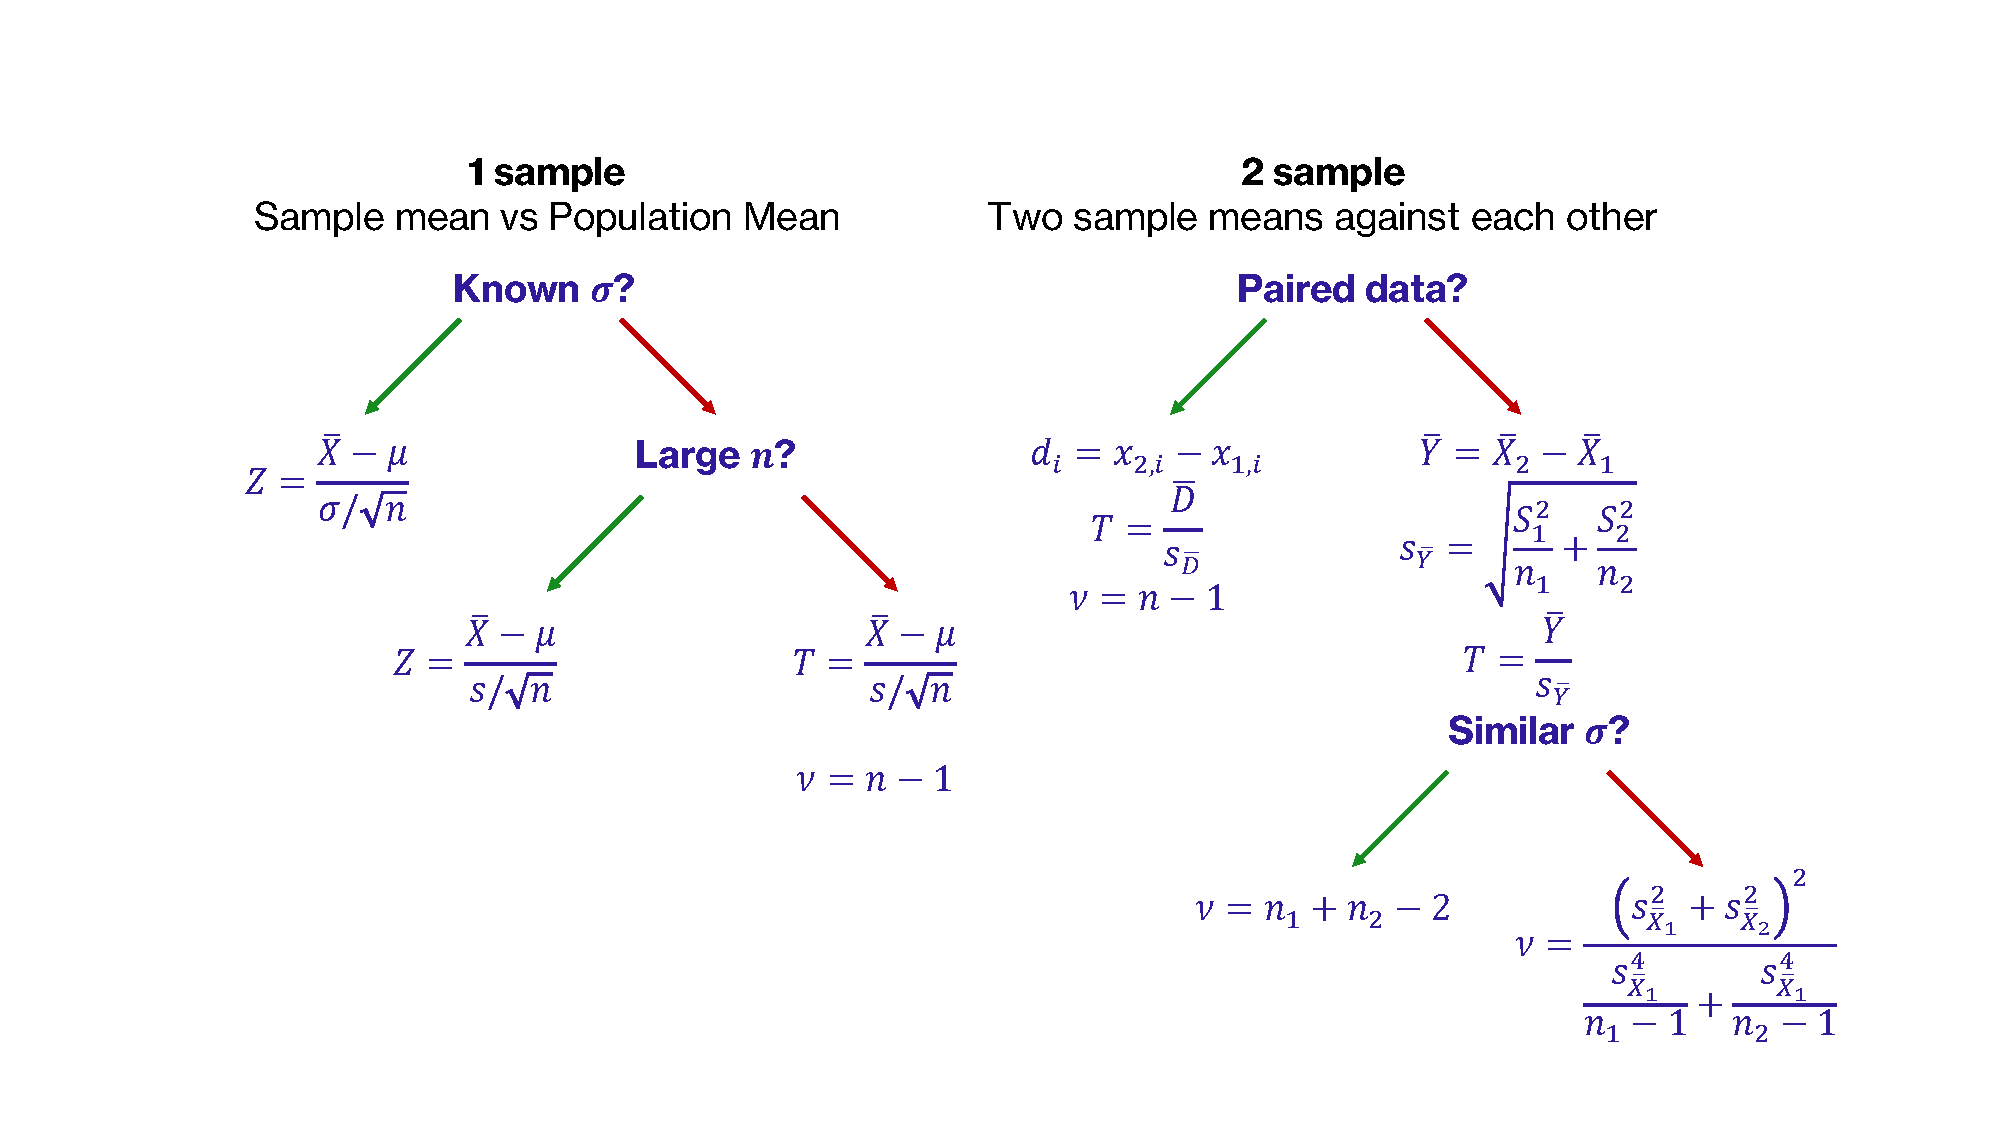
\includegraphics[width=.65\textwidth]{./images/zTest_and_tTest.pdf}
\end{figure}

%% 
\vspace{-2cm}
\subsection*{ANOVA}
Assumptions:
\begin{itemize}
\item{Data are sampled from a normal distribution. Often lognormal distribution is more appropriate (Use SW or AD test to confirm)}
\item{All groups have similar variance (homoscedastic) (Use Levene’s or Bartlett’s test to confirm)}
\item{Hypothesis $H_{0}$: no differences between the means of any of the groups}
\end{itemize}
%%
\subsection*{One-way ANOVA}
\begin{itemize}
    \item Sample means and grand mean: 
        \begin{table}[H]
        \centering
        \begin{tabular}{c|c}
        Sample Means & Grand Mean \\ \hline
        $\displaystyle \bar{X}_{i} = \frac{1}{J} \sum_{j=1}^{J}X_{i, j}$
        & 
        $\displaystyle \bar{X} = 
        \frac{1}{N}\sum^{I}_{i=1}\sum^{J}_{j=1}X_{i,j} = \frac{1}{I}\sum_{i=1}^{I}\bar{X}_{i}$\\
         \end{tabular}
        \end{table}
        \begin{itemize}
            \item $I$ denotes the number of groups
            \item $J_{i}$ denotes the number of observations for a given group. 
            \item $N$ is the total number of observations, $N = \sum_{i=1}^{I}J_{i}$.
            \item $X_{i,j}$ is a random variable that denotes the $j^{th}$ observation from the $i^{th}$ group.
        \end{itemize}
        
    \item Sums of Squares: $SS_{T} = SS_{R}+SS_{M}$
        \begin{table}[H]
        \centering
        \begin{tabular}{c|c|c|c}
        & Sum of Squares & DoF & Notes \\ \hline
        Total & $\displaystyle SS_{T} = \sum_{i=1}^{I}\sum_{j=1}^{J_{i}}(X_{i,j}-\bar{X})^{2}=(N-1)S_{grand}^{2}$ & $\displaystyle \nu_{T}=N-1$ & $\displaystyle S^{2}_{grand} = \frac{1}{N-1}\sum^{I}_{i=1}\sum_{j=1}^{J_{i}}(X_{i,j}-\bar{X})^{2} $\\ \hline

        Model & $\displaystyle SS_{M} = \sum^{I}_{i=1}J_{i}(\bar{X}_{i}-\bar{X})^{2}$ & $\displaystyle \nu_{M}=I-1$\\ \hline
         
        Residuals & $\displaystyle SS_{R} = \sum_{i=1}^{I}\sum_{j=1}^{J_{i}}(X_{i,j}-\bar{X}_{i})^{2}=\sum_{i=1}^{I}S_{i}^{2}(J_{i}-1)$ & $\displaystyle \nu_{R} = N-I$ & $\displaystyle S_{i}^{2} = \frac{\sum_{j=1}^{J_{i}}(X_{i,j}-\bar{X}_{i})^{2}}{J_{i}-1}$\\ 
         \end{tabular}
        \end{table}
   
   \item Mean square values and test-statistic:
   \[MS_{M} = \frac{SS_{M}}{\nu_{M}} = \frac{1}{I-1}\sum^{I}_{i=1}J_{i}(\bar{X}_{i}-\bar{X})^{2} \quad \quad \quad  MS_{R} = \frac{SS_{R}}{\nu_{R}} = \frac{1}{N-I} \sum_{i=1}^{I}\sum_{j=1}^{J_{i}}(X_{i,j}-\bar{X}_{i})^{2}\]
   \[F = \frac{MS_{M}}{MS_{R}} \quad \quad \quad p =1-f(F, \nu_{M}, \nu_{R})\]
\end{itemize}


\subsection*{Two-way ANOVA}
        \begin{table}[H]
        \begin{adjustbox}{width=\columnwidth,center}
        \begin{tabular}{c|c|c|c|c|c}
        & Sum of Squares & DoF & Mean Square & F-Statistic & Notes \\ \hline
        Total & $\displaystyle SS_{T} = \sum_{g=1}^{G}\sum_{i=1}^{I}\sum_{j=1}^{J}(X_{g,i,j}-\bar{X})^{2}$ & $\displaystyle \nu_{T}=N-1$ & & & $N=GIJ$\\ \hline

        Model & $\displaystyle SS_{M} = \sum_{g=1}^{G}\sum^{I}_{i=1}J(\bar{X}_{gi}-\bar{X})^{2}$ & $\displaystyle \nu_{M}=GI-1$ & & &\\ \hline
         
        Residuals & $\displaystyle SS_{R} = \sum_{g=1}^{G}\sum_{i=1}^{I}\sum_{j=1}^{J}(X_{g,i,j}-\bar{X}_{gi})^{2}$ & $\displaystyle \nu_{R} = N-GI$ & $\displaystyle MS_{R} = \frac{SS_{R}}{\nu_{R}}$ & & \\ \hline
         
        $SS_{A}$  & $\displaystyle SS_{A} = IJ \sum_{g=1}^{G}(\bar{X}_{g}-\bar{X})^{2}$ & $\displaystyle \nu_{A} = G-1$ & $\displaystyle MS_{A} = \frac{SS_{A}}{\nu_{A}}$ & $\displaystyle F_{A} = \frac{MS_{A}}{MS_{R}}$ & $SS_{M}$ grouped by G\\ \hline
         
        $SS_{B}$  & $\displaystyle SS_{B} = GJ \sum_{i=1}^{I}(\bar{X}_{i}-\bar{X})^{2}$ & $\displaystyle \nu_{B} = I-1$ & $\displaystyle MS_{B} = \frac{SS_{B}}{\nu_{B}}$ & $\displaystyle F_{B} = \frac{MS_{B}}{MS_{R}}$ & $SS_{M}$ grouped by I\\ \hline
         
        $SS_{A \times B}$  & $\displaystyle SS_{A \times B} = SS_{M}-SS_{A}-SS_{B}$ & $\displaystyle \nu_{A \times B} = \nu_{M}-\nu_{A}-\nu_{B}$ & $\displaystyle MS_{A\times B} = \frac{SS_{A\times B}}{\nu_{A\times B}}$ & $\displaystyle F_{A\times B} = \frac{MS_{A\times B}}{MS_{R}}$ & left over $SS$\\
         \end{tabular}
         \end{adjustbox}
        \end{table}
\begin{figure}[H]
    \centering
    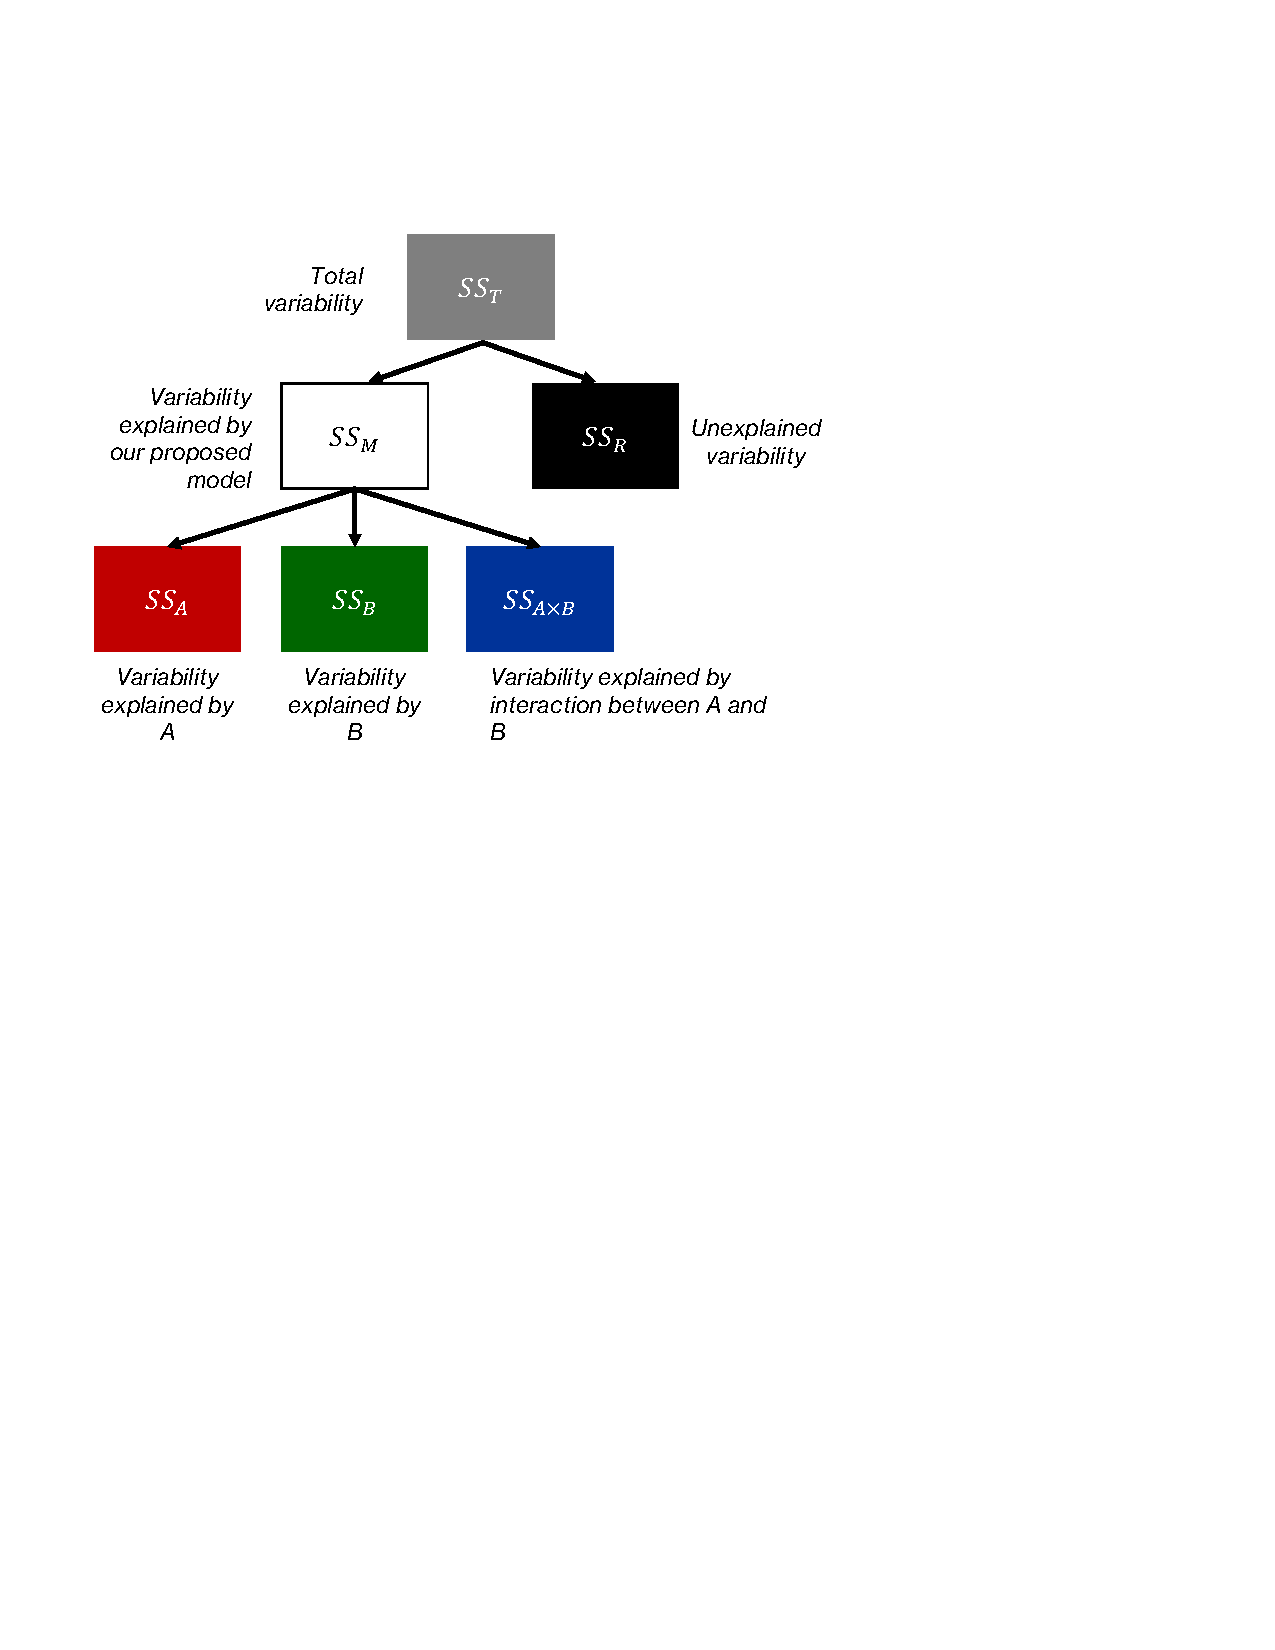
\includegraphics[width=.5\textwidth]{./images/twoWayANOVA.pdf}
\end{figure}
\subsection*{Post-Hoc Tests}
\begin{itemize}
            \item Bonferroni - pairwise t-tests. Statistically significant if $p < p_{crit}=\frac{\alpha}{I}$.
            \item Tukey Kramer Test (less conservative than Bonferroni).
        \end{itemize}
        
        
        
% =======================================================================
\subsection{Non-parametric Tests: \footnotesize{when data does not fit a known distribution}}
%%
\begin{figure}[H]
    \centering
    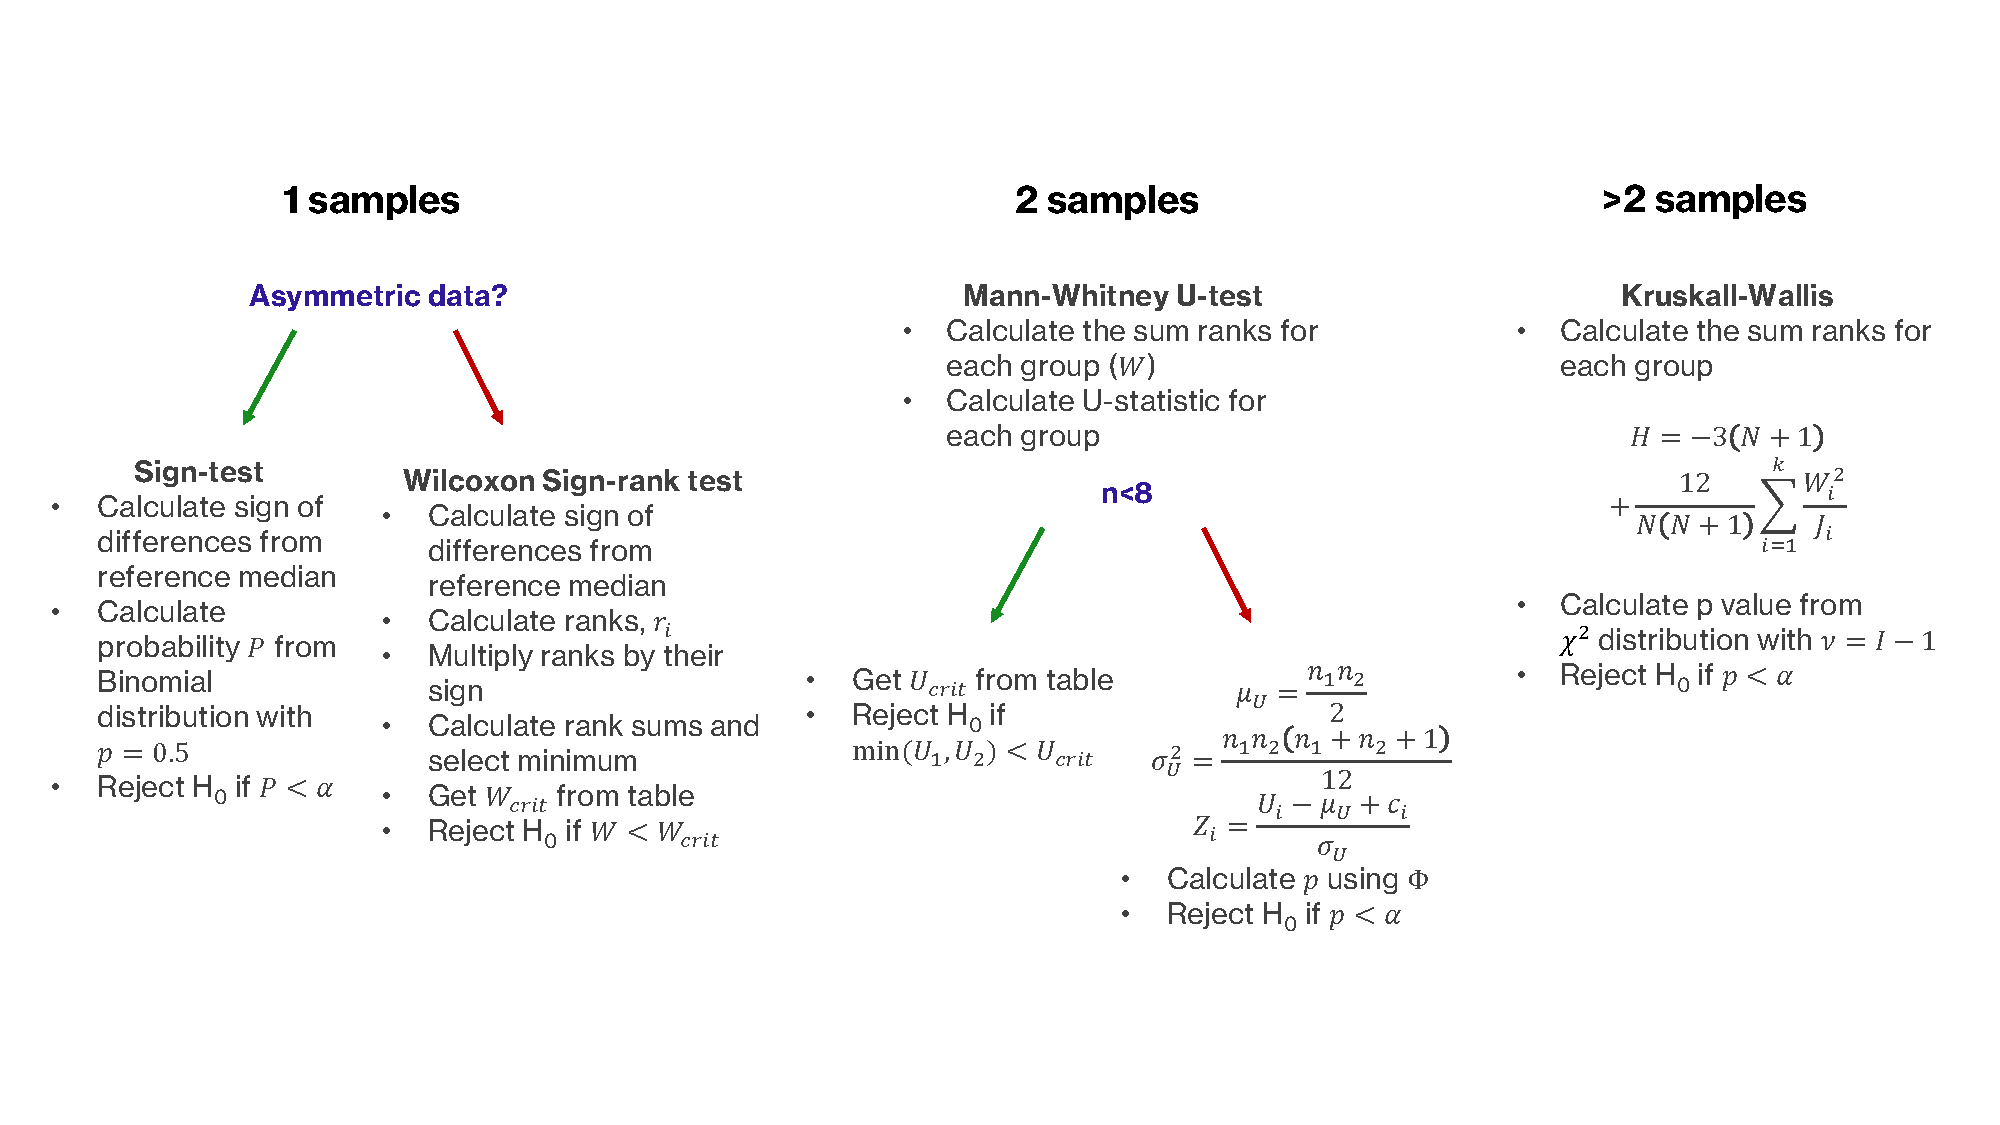
\includegraphics[width=\textwidth]{./images/nonparasummary.pdf}
\end{figure}
%%
\subsubsection{Sign test: \footnotesize{one sample, asymmetric data.}}
 \begin{itemize}
        \item Find the difference between each sample to a \textit{pre-defined} median value, $\tilde{\mu}_{0}$;
        \item Null hypothesis, $H_{0}$: the population median $\tilde{\mu}$ from which the sample is taken is equal to $\tilde{\mu}_{0}$.
        \item If $H_{0}$ is true, we should obtain at least $n/2$ of data points that are negative/positive.   
        \item Find $P$ by taking binomial test by taking $p=0.5$.  $\displaystyle b(x;n,p) ={ n \choose x} p^{x}(1-p)^{n-x}$
 \end{itemize}
%%
\subsubsection{Wilcoxon Sign-rank test: \footnotesize{one sample, non-symmetric data}}
\begin{itemize}
    \item Find the difference between each sample to a \textit{pre-defined} median value, $\tilde{\mu}_{0}$; Consider both the \textbf{sign} and \textbf{magnitude} of differences.
        \item Sort and find the rank of the differences. Multiply the ranks by their sign. 
        \begin{table}[H]
            \centering
            \begin{tabular}{l|c|c|c}
            rank  &  ...  &  ...&  ...\\ \hline
            $\lvert$difference$\rvert$ & ...  &  ...&  ...\\  \hline
            sign & ...  &  ...&  ...\\ \hline
            signed rank & ... &  ... &  ...\\ 
            \end{tabular}
        \end{table}
        \item calculate the absolute sum of the signed ranks, for +ve and -ve, respectively.
        \begin{itemize}
            \item $W^{+} = \sum_{i}^{n^{+}}R_{i}^{+}$ and $W^{-} = \sum_{i}^{n^{-}}-R_{i}^{-}$
            \item the smaller one becomes the test statistic.
        \end{itemize}
        \item Critical value $W_{crit}$ can be located from the table. 
\end{itemize}
%%
\subsubsection{Mann-Whitney U-test: \footnotesize{two samples}}
\begin{itemize}
        \item Make hypothesis: 
        \begin{itemize}
            \item $H_{0}$: the mean rank of the two levels are equal. (If samples are independent are from similar underlying distributions : mean rank -> median.)
            \item $H_{1}$: the mean rank of the two levels are different.
        \end{itemize}
        \item Group both samples, rank and correct averages \textbf{in one table}.
         \begin{table}[H]
            \centering
            \begin{tabular}{l|c|c|c}
            rank  &  ...  &  ...&  ...\\ \hline
            data value & ...  &  ...&  ...\\ 
            \end{tabular}
        \end{table}
        \item Calculate the sum ranks for each group $W$.
        \[W_{X}=\sum_{i}^{n_{X}}R_{i}^{X} \quad \quad W_{Y}=\sum_{i}^{n_{Y}}R_{i}^{Y}\]
        \item Calculate U-statistic for each group
        \[U_{i} = W_{i}-\frac{n_{i}(n_{i}+1)}{2}\]
        \item For $n<8$: $U_{crit}$ can be found from the table. Reject $H_{0}$ if $min(U_{1}, U_{2})<u_{crit}$
        \item For $n\geq 8$: \[\mu_{U}=\frac{n_{1}n_{2}}{2} \quad \quad \sigma_{U}^{2}= \frac{n_{1}n_{2}(n_{1}+n_{2}+1)}{12}\]
        z-statistic can be calculated by \[Z_{i}=\frac{U_{i}-\mu_{U}(+continuity)}{\sigma_{U}}\]
    \end{itemize}
%%
\subsubsection{Kruskall-Wallis test: \footnotesize{more than two samples}}
\begin{itemize}
        \item $H_{0}$: the $I$ independent random samples all come from identical populations.
        \item Calculate the sum ranks for each group: 
        \[H=-3(N+1)+\frac{12}{N(N+1)}\sum_{i=1}^{k}\frac{W_{i}^{2}}{J_{i}}\]
        \item For all $J_{i} > 5$, and if $H_{0}$ is true, $H$ is approximated to $\chi^{2}$ distribution with $\nu = I-1$.
\end{itemize}
%%


%%%%%%%%%%%%%%%%%%%%%%%%%%%%%%%%%%%%%%%%%%%%%%%%
\newpage
\section{Correlation and Regression}
\subsection*{Correlation}
\begin{table}[H]
    \centering
    \begin{adjustbox}{width=\columnwidth,center}
    \begin{tabular}{c|c}
    Covariance & Population \\
    (discrete and continuous)& Correlation Coefficient \\ \hline 
    $\displaystyle cov(X, Y)= E[(x-\mu_{X})(y-\mu_{Y})] 
    = E(XY)-E(X)E(Y)=\begin{cases}
    \displaystyle \sum_{x}\sum_{y}(x-\mu_{X})(y-\mu_{Y})p(x,y)\\
    \displaystyle \int_{-\infty}^{+\infty}\int_{-\infty}^{+\infty}  (x-\mu_{X})(y-\mu_{Y})f(x,y) dxdy %& continuous 
    \end{cases} $
     &  $\displaystyle \rho_{X,Y} = \frac{cov(X,Y)}{\sigma_{X}\sigma_{Y}}$\\ 
    \end{tabular}
    \end{adjustbox}
\end{table}
  \begin{itemize}
     \item \textbf{Pearson's correlation coefficient}: $r$ is an point estimator of $R = \hat{\rho}$.  Assume linear relationship between $X$ and $Y$. 
     \[\sigma_{X}^{2} = S_{XX} = \frac{\sum_{i=1}^{n}(x_{i}-\bar{x})^{2}}{n-1}, \quad \quad \sigma_{Y}^{2} = S_{YY} = \frac{\sum_{i=1}^{n}(y_{i}-\bar{y})^{2}}{n-1}, \quad \quad cov(x,y) = S_{XY} = \frac{\sum_{i=1}^{n}(x_{i}-\bar{x})(y_{i}-\bar{y})^{2}}{n-1}\]

    \[\Rightarrow \quad r_{X, Y} = \frac{S_{XY}}{\sqrt{S_{XX}}\sqrt{S_{YY}}} = \frac{\sum_{i=1}^{n}(x_{i}-\bar{x})(y_{i}-\bar{y})}{\sqrt{\sum_{i=1}^{n}(x_{i}-\bar{x})^{2}}\sqrt{\sum_{i=1}^{n}(y_{i}-\bar{y})^{2}}} \quad \in [-1, 1]\]
    
    \item \textbf{Test statistic and DoF}
    \[T = \frac{R\sqrt{n-2}}{\sqrt{1-R^{2}}}, \quad \quad \nu = n-2\]
     \item \textbf{Spearman's rank correlation coefficient}: non-linear relationship between $X$ and $Y$ -  $ \displaystyle \rho = 1- \frac{6\sum(x_{i}-y_{i})^{2}}{n(n^{2}-1)}$, where $x_{i}, y_{i}$ are ranks. If $x_{i}, y_{i}$ are tied, we evaluate Pearson's $r$ on the ranks.
  \end{itemize}
  %%
 
\subsection*{Regression}
\begin{itemize}
    \item \textbf{Regression model} - $Y = b_{0} + b_{1}X + \epsilon$, where $\epsilon$ is a normally distributed random variable with $E(\epsilon) = 0$ and $V(\epsilon) = \sigma_{\epsilon}^{2}$.
    \item \textbf{Estimate of the best fit line}
    
    \begin{minipage}{.45\textwidth}
    \begin{table}[H] \centering
    \begin{tabular}{c|c|c}
    \multicolumn{3}{c}{$\mathbf{Y=\hat{b}_{0}+\hat{b}_{1}X}$}\\ \hline
    slope & $\displaystyle \hat{b}_{1} = \frac{S_{xy}}{S_{xx}}$ & $\displaystyle s_{\hat{b}_{1}} = \frac{s_{\epsilon}}{\sqrt{S_{xx}}}$\\ \hline
    intercept & $\displaystyle \hat{b}_{0} = \bar{y}-\hat{b}_{1}\bar{x} $ & $\displaystyle s_{\hat{b}_{0}} = \sqrt{\frac{1}{n}+\frac{\bar{x}^{2}}{S_{xx}}}$
    \end{tabular}\end{table}
    \end{minipage}
    \begin{minipage}{.05\textwidth}\[\xrightarrow{\text{with}}\]
    \end{minipage}
    \begin{minipage}{.45\textwidth}
    \begin{tabular}{c|c|c} \centering
    $S_{xx}$ & $S_{yy}$ & $S_{xy}$ \\ \hline
    $\displaystyle \sum_{i=1}^{n}(x_{i}-\bar{x})^{2}$ & $\displaystyle \sum_{i=1}^{n}(y_{i}-\bar{y})^{2}$ & $\displaystyle \sum_{i=1}^{n}(x_{i}-\bar{x})(y_{i}-\bar{y})$ 
    \end{tabular}\end{minipage}
    \begin{itemize}
        \item Best estimator for variance of residuals -  $\displaystyle \hat{\sigma}_{\epsilon}^{2} = s_{\epsilon}^{2} = \frac{SS_{R}}{\nu_{R}} = \frac{\sum_{i=1}^{n}(y_{i}-\hat{y}_{i})^{2}}{n-2}$
    \end{itemize}
    
    \item \textbf{Coefficient of determination}: \[r^{2} = 1-\frac{SS_{R}}{SS_{T}}, \quad \quad \text{where} \quad SS_{T}=S_{yy}, \quad SS_{R}=s_{\epsilon}^{2}\nu_{R}, \quad \quad \]
    
    \item \textbf{Confidence interval}:
     \begin{table}[H] \centering
    \begin{tabular}{c|c|c}

   slope & intercept & variance of residual \\ \hline
   $CI=\hat{b}_{1} + t_{1-\frac{\alpha}{2}, \nu}s_{\hat{b}_{1}}$ & $CI=\hat{b}_{0} + t_{1-\frac{\alpha}{2}, \nu}s_{\hat{b}_{0}}$ &
   $s_{\epsilon}^{2}= SS_{R}/\nu_{R}$ and $\nu_{R}=n-2$
    \end{tabular}\end{table}
    
    \item \textbf{Confidence bands}: For any given value of $x^*$, uncertainty on the mean
    \[CI = \hat{y}^{*}\pm t_{\frac{\alpha}{2}, n-1}s_{\hat{y}^{*}} \quad \quad s_{\hat{y}^{*}} = s_{\epsilon}\sqrt{\frac{1}{n}+\frac{(x^{*}-\bar{x})^{2}}{\sum_{i=1}^{n}(x_{i}-\bar{x})^{2}}}\]
    
    \item \textbf{Prediction bands}: uncertainty on a single measurement
    \[s_{pred}^{2} = s_{\hat{y}^{*}}^{2} + s_{\epsilon}^{2} \quad \quad PI=\hat{y}^{*}\pm t_{\frac{\alpha}{2}, n-2} s^{*}_{pred}\]
\end{itemize}
 

% footer by framebox, auto update
\vspace*{\fill}
\framebox{\footnotesize Scripted by B Li \& P Xie. \ Last update: \today}

% attach the Z-t-F data tables
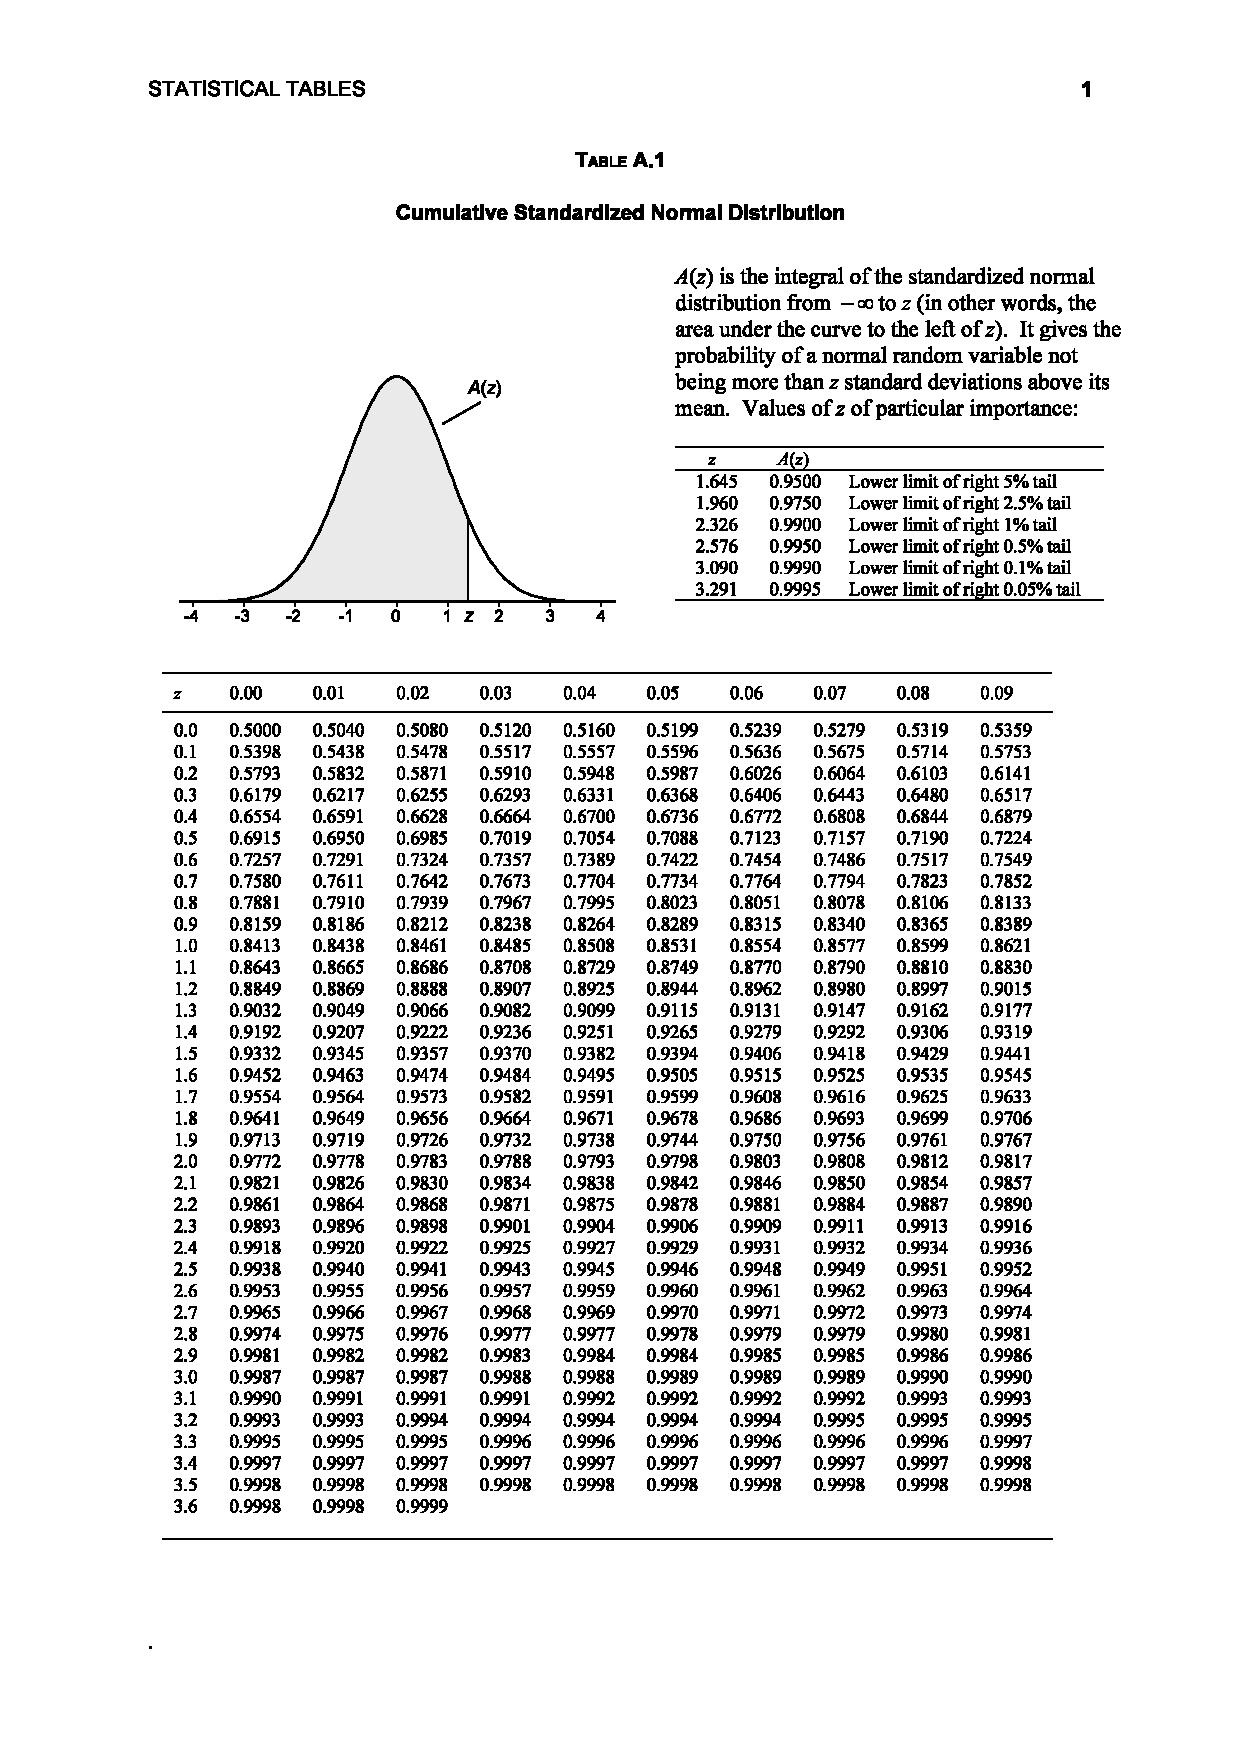
\includepdf[pages=-]{./images/Z_t_F_Tables.pdf}

% end the doc
\end{document}